\section{Real-time implementation and preliminary results}
\label{sec:rt}

The application consists of a
static GTFS~schedule and network data component,
and a \rt modeling and prediction component.
We chose \verb+Rcpp+ to develop the program,
providing access to other R packages for data manipulation 
(notably \verb+RSQLite+ and \verb+dplyr+),
as well as the speed and memory management capabilities of \verb|C++|. 
The following has been implemented in the R package
\verb+transitr+, available on Github (\url{https://github.com/tmelliott/transitr}).
In this section, we discuss the features of the \rt component.

The general structure of the \rt component is:
\begin{enumerate}
\item Load GTFS data from database
\item Indefinitely repeat when new data recieved \ldots
\begin{enumerate}
    \item Update or create new vehicle objects from new data
    \item Run particle filter on each vehicle to estimate update state
    \item Collect travel time information for each vehicle for any completed roads
    \item Update road network for any completed road segments
    \item Generate ETAs for vehicles uing combination of particle filter and network state
    \item Write ETAs to extended Google Protobuf binary file for distribution
\end{enumerate}
\end{enumerate}


During the development of the application,
we were primarly concerned with ensuring each component of the program
is as efficient as possible,
allowing ETAs to be generated and distributed fast enough---our initial goal was 30~seconds.
Using \verb|C++| provides enough control over memory management
to ensure the program runs fast enough in \rt 
while still implementing the models.
We could also use OpenMP for parallelisation,
allowing us to process multiple vehicles simultaneously
depending on the number of cores available.


The particle filter requires thousands of particles per vehicle,
so it is necessary to explore the performance of the application
with varying number of particles.
It is also necessary to assess the performance of the particle filter,
and compare values for the fixed model parameters.
To do so, we implemented a simulated \rt environment
in which we could analyse the same subset of real vehicle data from 8~October, 2018
using a range of settings.
These simulations were carried out of a Virtual Machine 
with 8~cores and 32~Gb of memory, 
running Ubuntu~16.04 and using R~3.4.1.

\begin{figure}[tb]
    \centering
    % \includegraphics[width=0.7\textwidth]{figures/04_model_results_gps.pdf}
    \caption{The distance between the observation and the nearest point on the shape.}
    \label{fig:gps_dist}
\end{figure}



\subsection{Program Timings}
\label{sec:timings}

During development of our application,
our primary concert was the computational faesibility of a particle filter.
For each iteration, 
the timings of the individual components in 2a--f above are recorded.
Since the number of vehicles traveling at any given time changes throughout the day,
we used the average timings over a 15~minute window to compare.


Figure~\ref{fig:timings} shows the timing results for varying number of particles.
We see that there is a very slight quadratic trend to run times,
as several steps are not of complexity $O(N)$,
the main one being the estimation of ETA quantiles.
While not discussed in this paper,
the application generates ETAs for each particle
and calculates ETA quantiles for each vehicle to demonstrate the computational faesibility.
This step requires sorting a vector, which is $O(N\log(N))$.
Clearly, our initial target of 30~seconds is obtainable given the number of particles
is not too large, and there are enough cores.


\begin{figure}[tb]
    \centering
    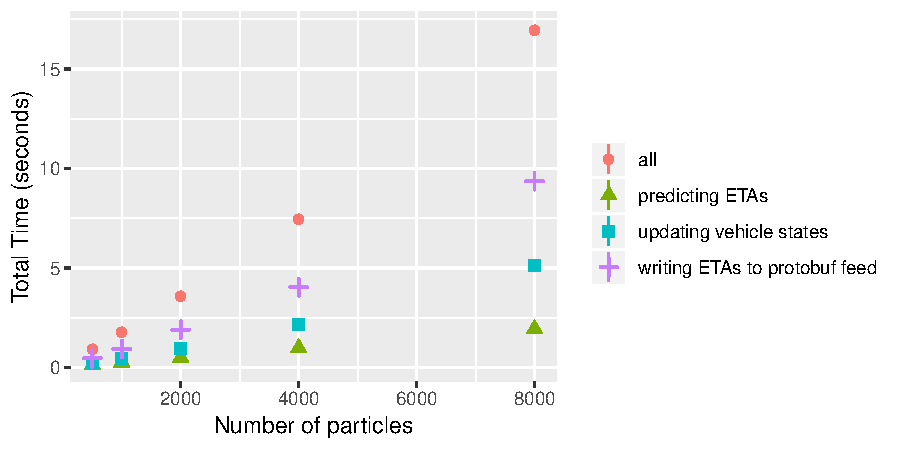
\includegraphics[width=0.7\textwidth]{figures/04_model_results_timing.pdf}
    \caption{The timings for various parts of the application, and overall. %
        The trend is slightly non-linear due to the complexity of the ETA generation step, %
        which requires sorting of the particle ETAs to obtain quantile estimates.}
    \label{fig:timings}
\end{figure}




\subsection{Model performance}
\label{sec:model_perf}


The parameters varied were the number of particles,
GPS error $\epsilon$, and system noise $\sigma^2$.
The primary goal is to reduce the rate of degeneration and ``losing'' the bus 
(i.e., no particles are near the observed location),
and reducing the variance of parameter estimates; here we use vehicle speed as the example.


The one parameter we can determine from the data is GPS error, $\epsilon^2$,
by looking at the distance between observations and the shape.
Figure~\ref{fig:gps_dist} shows the distribution of distance between the vehicle
observation and the \emph{nearest point on the path}.
Due to the way the observations are reported, 
many observations will be ``exactly'' on the route at a bus stop,
and we need to ignore these.


To check the model results, 
we need to realise that we are not trying to accurately predict
future locations of the vehicle,
but instead are trying to use a sequence of GPS positions to infer travel
times along intermediate roads.
Therefore, several tools used to assess the validity of a particle filter
are unnecessary.
Instead, we will be comparing the rate of degeneration 
(i.e., the particle sample loses the actual bus and needs to be reinitialized)
and the mean distance between the state estimate and the observation; 
we will use the distance between the observation and the route (cross track distance) 
to determine how well the posterior distribution fits the data---%
if the ratio between the CTD and RMSE is large,
then the fit is ``bad''.
[We also explore the uncertainty of travel time estimates,
as well as the variability between consecutive buses]\footnote{assuming we can get the results in time}.

\begin{figure}[tb]
    \centering
    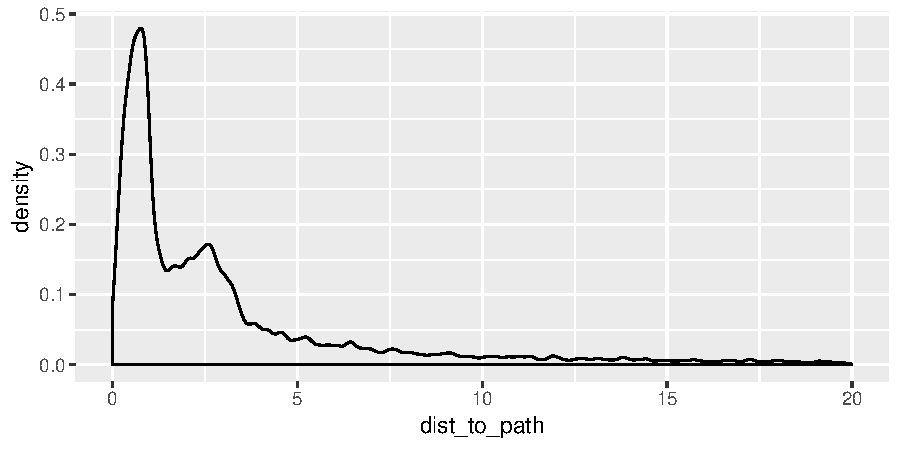
\includegraphics[width=0.7\textwidth]{figures/04_model_results_dist.pdf}
    \caption{The timings for various parts of the application, and overall. %
        The trend is approximately linear with the number of particles.}
    \label{fig:dist_to_route}
\end{figure}

\begin{figure}[tb]
    \centering
    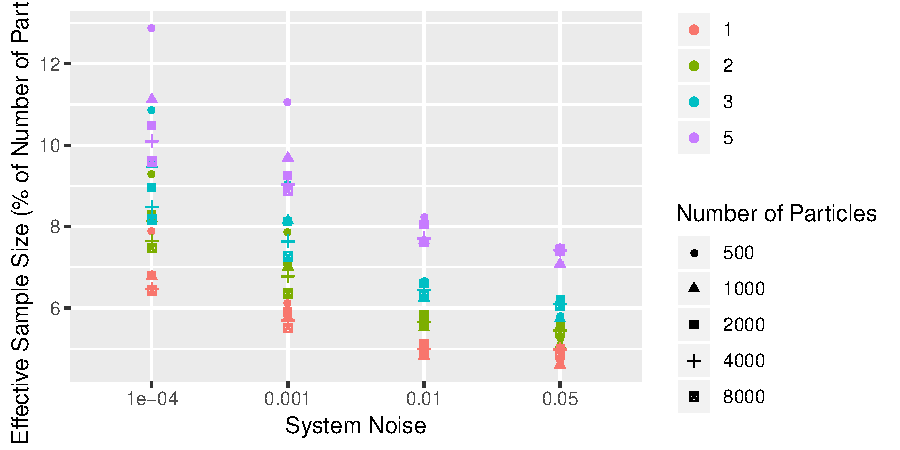
\includegraphics[width=0.7\textwidth]{figures/04_model_results_neff.pdf}
    \caption{The timings for various parts of the application, and overall. %
        The trend is approximately linear with the number of particles.}
    \label{fig:neff}
\end{figure}




From the Figure~X, 
we see a trade-off between some of the parameters.
Larger values of GPS error decrease the degeneration rate
as well as the rate of resampling (which increases speed);
however, the cost of this is that the mean distance between the posterior distribution
and the observed location increases, giving a less precise estimate of the vehicle's state.
Conversely, the system noise does not have the same effect,
and only slightly effects the values.





% How we implement it, choice of software (Rcpp = R + C++).
% R: dealing with data structures is easier, maintainability, interfacing
% C++: speed

% Overall structure:
% - load
% - fetch positions
% - initialize or mutate+update
% - update network
% - make ETA predictions (vehicle state + network state)

% Some of the key things:
% - minimise copy, parallelisation using OMP
% - moving as much computation ``outside'' of the main loop as possible
%   (e.g., ``pre''-predict vehicle/network states so only update required)
%   so ETAs are generated ASAP after retrieving data
% - keeping the GTFS database up-to-date by fetching new data each morning
% - distribution - a cloud database vs a single protobuf file with everything 
%   (maintenance/reliability/speed/size)

